\documentclass[11pt,a4paper]{article}
\usepackage[T1]{fontenc}\usepackage[utf8]{inputenc}\usepackage[provide=*,danish]{babel}
\usepackage{lmodern,amsmath,amssymb,geometry,hyperref,microtype,graphicx}
\geometry{margin=25mm}\setlength{\parindent}{0pt}\setlength{\parskip}{6pt}\setlength{\emergencystretch}{3em}
\hypersetup{colorlinks=true,urlcolor=blue}
\title{Generel ECD: kollaps, bounce og e-folds\\\large Eksakte relationer, målemetoder og åbne problemer}
\author{Skovlab}\date{14. november 2026}
\begin{document}\maketitle
\textbf{Hvad undersøgelsen kan give.} Vi undersøger minimal klassisk Einstein--Cartan--Dirac (ECD) uden homogenitet, isotropi eller rumlig symmetri. Vi fastlægger e-folds for strøm, snitvolumener og forskellige retninger, udleder generelle regularitetskrav og tilføjer passiv sporing til den eksisterende 3D-motor. Der er ikke ét universelt bounce eller e-foldtal, som actionen alene bestemmer. En fuldstændig klassifikation af alle globale ECD-løsninger er ikke leveret.

\section{Den generelle teori inden for en fastlagt action}
Vi bruger signaturen $(-+++)$, $\kappa=8\pi G$, fuld torsion $T^a{}_{bc}=2\widetilde\Gamma^a{}_{[bc]}$ og projektets korrigerede Clifford-/spinforbindelseskonventioner. Efter algebraisk elimination af torsion er actionen for flere klassiske Dirac-felter
\[
 S=\int e\left[\frac R{2\kappa}+\sum_f\mathcal L_{D,f}^{\circ}-G_A A_aA^a\right]d^4x,
 \quad G_A=\frac{3\kappa}{16},\quad
 A^a=\sum_f\bar\psi_f\gamma_5\gamma^a\psi_f.
\]
Her er $\{\gamma^a,\gamma^b\}=-2\eta^{ab}$, $\bar\psi=\psi^\dagger\gamma^0$ og $\gamma_5=-i\gamma^0\gamma^1\gamma^2\gamma^3$. Med geometrisk frameforbindelse $W$ bruges $D=\partial-W^{ab}[\gamma_a,\gamma_b]/8$. Den fulde torsion er $T_{abc}=-\kappa\epsilon_{abcd}A^d/2$. Der tilføjes ingen selvstændigt propagerende torsion, ekstra væske eller bouncekraft.

Feltligningerne er
\[
 i\gamma^\mu D_\mu\psi_f-m_f\psi_f-2G_A A_a\gamma_5\gamma^a\psi_f=0,
 \qquad G_{\mu\nu}=\kappa T_{\mu\nu},
\]
\[
 T_{\mu\nu}=\sum_f\mathcal K^{(f)}_{\mu\nu}+G_Ag_{\mu\nu}A^2,\qquad
 \mathcal K^{(f)}_{\mu\nu}=-\frac i4[\bar\psi_f\gamma_\mu\overleftrightarrow D_\nu\psi_f+
 \bar\psi_f\gamma_\nu\overleftrightarrow D_\mu\psi_f].
\]
Torsionskvadratet omfatter også krydsled mellem arter. Den eksisterende 3D-motor implementerer ét felt; flertalsligningerne er en præcis teoretisk udvidelse, ikke en leveret kvantegas-solver.

ADM-geometrien
\[
 ds^2=-N^2dt^2+\gamma_{ij}(dx^i+\beta^idt)(dx^j+\beta^jdt)
\]
kræver rumlig metrik, ekstrinsisk krumning $K_{ij}$, alle spinorkomponenter samt gauge, topologi og rand-/asymptotiske data. De fire Einstein-constraints skal være opfyldt. Masse, radius, spintryk og kollapshastighed er derfor ikke frie, uafhængige væskeinput. Ligningerne er klassisk lukkede efter datavalg; det giver ikke automatisk et numerisk stabilt eller globalt fuldstændigt kollapsproblem.

\section{Lokale e-folds uden FLRW}
Vælg en timelig, ikke-nul bevaret strøm $j^\mu=n u^\mu$. Den normaliserede hastighed er $u^2=-1$ og $n=\sqrt{-j^2}$. Strømbevarelse giver
\[
 \nabla_\mu j^\mu=0\quad\Longrightarrow\quad \dot n=-n\Theta_u,
 \qquad\Theta_u=\nabla_\mu u^\mu.
\]
Prikken er afledt langs strømmen i egentid. For et fulgt infinitesimalt hvilevolumen er $\dot v_u/v_u=\Theta_u$. Derfor
\[
 \boxed{N_u=\frac13\int\Theta_u\,d\tau
 =\frac13\ln(v_u/v_{u0})=-\frac13\ln(n/n_0).}
\]
Dette kræver ingen homogenitet, rotationsfrihed eller perfekt væske. Referencen og strømmen skal være erklæret. Ved nul eller null-strøm er denne hvileramme ikke defineret; det er ikke i sig selv en krumningssingularitet.

Positive e-folds betyder ekspansion, negative kontraktion. Én e-fold giver en faktor $e$ i den lokale volumenbaserede længdeskala, $e^3$ i volumen og $e^{-3}$ i strømtætheden. En cyklus med samme slut- og starttæthed har nul netto-e-folds, selv om både kontraktion og ekspansion var store. Vi registrerer derfor også særskilt
\[
 N_+=\int\max(\Theta_u/3,0)d\tau,\qquad
 N_-=-\int\min(\Theta_u/3,0)d\tau,
 \qquad N_{\rm net}=N_+-N_-.
\]
Energitætheden har ikke generelt samme simple lov som $n$. Den fulde ECD-stress kan have energiflux og anisotrop spænding; disse giver ekstra led i energibevarelsen. En klassisk strømtæthed er heller ikke automatisk et fysisk kvantepartikelantal i en tilstand med pardannelse.

\section{Normaler, tilt og retningsbestemt deformation}
ADM-normalernes ekspansion er $\Theta_n=-K$ med $H_n=-K/3$. Stoffet kan bevæge sig i forhold til dem. Sæt $W=-u\cdot n_{\rm ADM}=Nu^0$. Da gælder
\[
 \frac{dx^i}{dt}=\frac{j^i}{j^0},\quad
 \frac{d\tau}{dt}=\frac N W,\quad
 \frac{dN_u}{dt}=\frac{N\Theta_u}{3W}.
\]
Normalbanerne har derimod hastighed $-\beta^i$ og egentid $Ndt$, så deres e-folds er $N_n=-\int NK\,dt/3$ langs disse baner. Et metrikdeterminantforhold ved faste koordinater giver ikke generelt dette mål.

Lad $J^i{}_A=\partial x^i/\partial X^A$ være Jacobianen for fulgte strøm-etiketter. Volumenet på ADM-snittet er $v_\Sigma=\sqrt\gamma\det J\,d^3X$. Strømmen gennem det er $dQ=nWv_\Sigma$, og hvilevolumenet er $v_u=Wv_\Sigma$. Derfor
\[
 \boxed{N_\Sigma=N_u-\frac13\ln(W/W_0).}
\]
De to volumener og deres tidsmål skal holdes adskilt. Med rotation findes der normalt ikke én global hypersurface ortogonal til hele stofstrømmen.

De rumlige nabobaner opfylder den geometriske ligning
\[
 \frac{dJ^i{}_A}{dt}=\partial_j(j^i/j^0)J^j{}_A.
\]
Den er en målemetode, ikke en ny spintransportlov. Den hvileprojicerede rumlige metrik er $H^u_{ij}=\gamma_{ij}+u_i u_j$, med $\det H^u=W^2\det\gamma$. Jacobianen og denne metrik giver tre hovedstrækninger $\lambda_i^{1/2}$ og e-folds $N_i=\ln\lambda_i/2$. Deres gennemsnit er $N_u$. En retning kan stadig kontrahere, når gennemsnittet er positivt. Man kan ikke blot integrere øjeblikkelige shear-eigenværdier, hvis akserne roterer.

Et endeligt domæne har et særskilt mål $N_{D,\Sigma}=\ln(V_D/V_{D0})/3$ på en valgt slicing. Det er ikke det uvægtede gennemsnit af lokale log-volumener, og det har ikke automatisk én fælles egentid. Den nye kode følger lokale elementer; den konstruerer ikke en konvergeret hel skyvolumen.

\section{En generel regularitetstest for ét klassisk spinorfelt}
For én regulær kommuterende spinor giver Fierz-identiteten $A^2=n^2=S^2+\Pi^2$, altså $|S|\leq n$, hvor $S=\bar\psi\psi$. Den fulde stress og Dirac-ligningen giver
\[
 T^\mu{}_{\mu}=-mS+2G_A n^2,\qquad
 \boxed{R=\kappa mS-2\kappa G_A n^2.}
\]
Her er $R$ metrikforbindelsens Levi--Civita-Ricci-skalar. Den rumlige kinetiske stress er allerede elimineret fra sporet; den kan ikke vælges til at ophæve det led. For fast endelig masse følger derfor
\[
 \lim_{n\to\infty}R/n^2=-2\kappa G_A<0.
\]
Samtidig er torsionsinvarianten
\[
 T_{abc}T^{abc}=-\tfrac32\kappa^2n^2.
\]
Hvis den bevarede strøm fortsat komprimeres med $N_u\to-\infty$, divergerer altså både metrikkens Ricci-skalar og torsionsinvarianten. Ved endelig egentid er det en invariant hindring for regulær fortsættelse. Hvis grænsen kun nærmes ved uendelig egentid, følger endelig-tids-geodætisk inkomplethed ikke af denne beregning alene.

Det viser ikke, at enhver sky når nulvolumen. Et bounce eller en anden udvikling kan forhindre det; klassisk gyldighed kan også svigte tidligere. ECD garanterer blot ikke automatisk, at torsion fjerner singularitetsmuligheden.

Det er vigtigt at kontrollere flere invarianter. Den fulde forbindelses skalar kan nemlig være
\[
 \widetilde R=R+3\kappa^2n^2/8=\kappa mS.
\]
For et masseløst felt kan denne ene skalar være nul, selv om metrik-Ricci og torsion divergerer. En ophævelse i én skalar er ikke fuld regularitet. Tilsvarende kan vakuum have $R=0$ og alligevel divergent Weyl-/Kretschmannkrumning.

Hvis man kræver $|R|\leq R_*$, fås nødvendigvis
\[
 n\leq n_{\max}=\frac{m+\sqrt{m^2+8G_A R_*/\kappa}}{4G_A},\qquad
 N_u\geq-\frac13\ln(n_{\max}/n_0).
\]
Det er en nødvendig regularitetsgrænse, ikke en forudsagt bouncedensitet. $R_*$ skal begrundes; en valgt numerisk stopværdi er ikke en fysisk overgang.

\section{Hvor generelt gælder det for flere felter og kvantestof?}
For flere felter gælder fortsat
\[
 R=\kappa\sum_fm_f\bar\psi_f\psi_f-2\kappa G_A A_{\rm tot}^2,
\]
men $A_{\rm tot}^2$ er ikke generelt den samlede strømtæthed i anden. Modsatte spin kan ophæve hinanden, og forskellige strømrammer giver yderligere frihed. Den enkle tæthedsbaserede regularitetsgrænse må derfor ikke overføres automatisk.

E-foldidentiteten gælder stadig for en valgt timelig bevaret totalstrøm, men torsionskildens skalering følger ikke alene af dette. For ét regulært klassisk felt er $A^2/A_0^2=e^{-6N_u}$ eksakt; for flere felter kræves de faktiske polariseringer og krydskorrelationer.

Kvantestatistisk stof kræver en tilstand, renormaliseret stress og sammensatte operatorer. $\langle A^2\rangle_{ren}$ er ikke generelt $\langle A\rangle^2$. Degenerationspres, stærke, svage og elektromagnetiske vekselvirkninger kommer ikke automatisk med i denne klassiske action. De tidligere materierapporter beskriver disse mangler. Ingen kvantegaslukning opfindes her.

\section{Bounce og antal e-folds er forskellige spørgsmål}
Raychaudhuri giver generelt
\[
 \dot\Theta=-\Theta^2/3-\sigma_{ab}\sigma^{ab}+\omega_{ab}\omega^{ab}
 -\frac\kappa2(\epsilon+3P)+\nabla_a a^a.
\]
Et lokalt bounce kræver en positiv højreside ved nul ekspansion samt regulær fortsættelse. Det tidligere analytiske eksempel opfylder dette for særlige constrainedata, men bryder en nulenergibetingelse og vender også i torsionsfri Einstein--Dirac. Det fastlægger ikke realistisk torsionsdrevet kollaps.

For det konkrete eksempel kender vi kun den lokale begyndelse af e-foldudviklingen:
\[
 N_u(\tau;0)=\frac{287}{576}m^2\tau^2+O(\tau^3).
\]
Denne Taylorserie giver ingen kontrolleret varighed og må ikke forlænges til et vilkårligt stort e-foldtal. En lille masse skalerer tiden, men skaber ikke af sig selv mange dimensionsløse e-folds.

Positivt $N$ er heller ikke bevis på inflation. Lokalt accelereret volumenekspansion kræver $H_u>0$ og $\dot H_u+H_u^2>0$, og en kosmologisk inflationspåstand kræver mere global geometri og horisonthistorie. Den sædvanlige størrelse $-\dot H/H^2$ er udefineret lige ved et bounce.

\section{Et eksakt torsionsdrevet kosmologisk bounce}
Vi har desuden verificeret en særlig løsning med seks uafhængige masseløse klassiske felter med samme kiralitet og lige store modsatrettede impulser langs tre akser. På en rumligt flad FLRW-metrik summerer deres fulde stress til en isotrop kilde uden statistisk gennemsnit. De enkelte felter er ikke rotationsinvariante. Totalstrømmen er timelig, mens den samlede aksialstrøm er timelig med $A^2=-n^2$. Dette er netop en mulighed, som ét regulært klassisk felt ikke har.

Direkte substitution i Dirac-ligningen og den fulde stress giver
\[
 \epsilon=C_r a^{-4}-C_s a^{-6},\quad
 P=\tfrac13 C_r a^{-4}-C_s a^{-6},\quad
 C_r=pn_0,\quad C_s=G_A n_0^2.
\]
Dette er afledte kildeudtryk for den erklærede felttilstand, ikke en antaget væskelukning. Med $a_b^2=C_s/C_r$ og $q^2=\kappa C_r/3$ er den eksakte løsning i konform tid
\[
 \boxed{a(\eta)=\sqrt{a_b^2+q^2\eta^2}},\qquad
 t(\eta)=\tfrac12\left[\eta a(\eta)+\frac{a_b^2}{q}
 \operatorname{arsinh}(q\eta/a_b)\right].
\]
Ved $\eta=0$ er $H=0$ og $\dot H>0$. Metrikkens krumning og torsion er begrænsede; løsningen er kausalt geodætisk komplet. Den torsionsfri Einstein--Dirac-reference med samme komovende ladninger og impulser kollapser derimod som stråling til $a=0$ i endelig egentid. Constraints løses særskilt i referencen. Bouncet er derfor reelt torsionsdrevet inden for denne særlige klassiske familie.

Efter bouncet er $N=\tfrac12\ln[1+(q\eta/a_b)^2]$. Accelerationen er positiv netop indtil $a=\sqrt2 a_b$, så
\[
 \boxed{N_{\mathrm{acc}}=\tfrac12\ln2\simeq0{,}346574.}
\]
Den senere ekspansion fortsætter ubegrænset, men er decelereret. Uendelige samlede fremtidige e-folds er således ikke uendelig inflation. Nulenergibetingelsen brydes indtil $N=\tfrac12\ln(3/2)$.

\textbf{Fysisk begrænsning.} Eksemplet er et kosmologisk rum med periodiske rumretninger, ikke en afgrænset sky med sort-hul-yderside. En illustrativ normalisering med én fermion pr. art i den fundamentale impulsmode giver $\kappa^2\rho_b=1024\pi^3/27\simeq1176$. Den ligger uden for en kontrolleret klassisk lavenergiforudsigelse. Vilkårlig stor klassisk feltbesættelse er ikke en Pauli-kompatibel kvantetilstand. Kvantekorrelationer, realistiske vekselvirkninger og perturbativ stabilitet er ikke afgjort af løsningen.

\IfFileExists{chiral-benchmark.png}{\begin{center}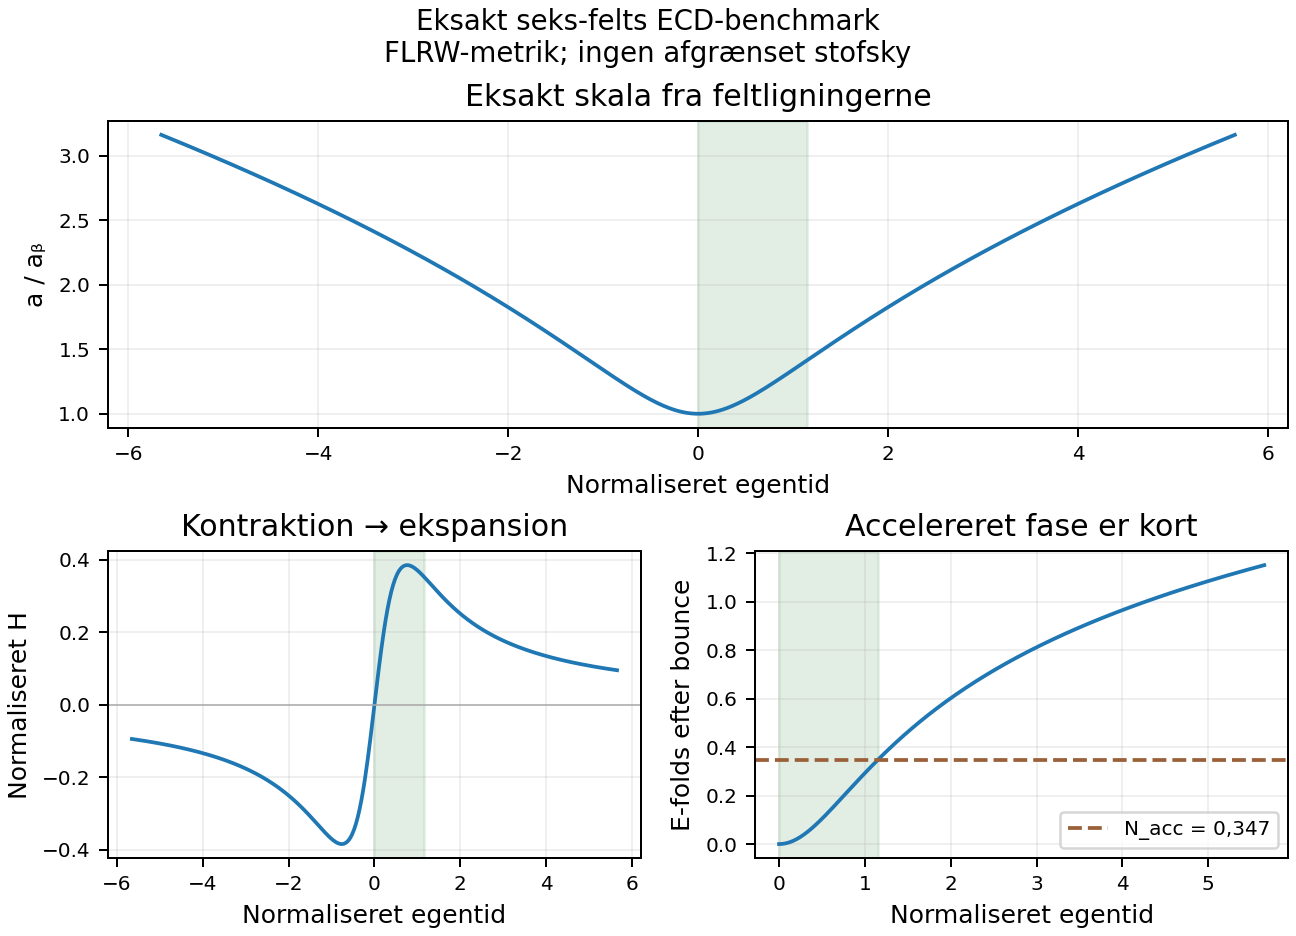
\includegraphics[width=\linewidth]{chiral-benchmark.png}\end{center}}{}

\section{Nødvendige grænser ved vedvarende positiv Ricci-skalar}
For ét felt er $R\leq\kappa mn-2\kappa G_A n^2\leq2m^2/3$. Hvis $R\geq R_{\min}>0$ gennem en fase, skal $m>0$ og
\[
 n_-\leq n\leq n_+,\quad
 n_\pm=\frac{m\pm\sqrt{m^2-8G_A R_{\min}/\kappa}}{4G_A},\quad
 N_{\rm net}\leq\tfrac13\ln(n_+/n_-).
\]
Dette er nødvendige sporgrænser, ikke en eksistenssætning eller en generel inflationsgrænse. De begrænser ikke summen af positive bidrag over gentagne cykler. For endeligt mange klassiske felter giver de fremtidige kausale kirale strømme $|A_{\rm tot}^2|\leq n_{\rm tot}^2$ og $|\sum m_f S_f|\leq m_{\max}n_{\rm tot}$. Derfor går $|R|\leq\kappa m_{\max}n_{\rm tot}+2\kappa G_A n_{\rm tot}^2$ mod nul ved ubegrænset strømekspansion. Det udelukker en vedvarende positiv Ricci-undregrænse i denne grænse, men udelukker ikke decelereret ekspansion som i eksemplet ovenfor.

\section{Hvad den nye 3D-sporing faktisk måler}
Den passive kode bruger præcis de eksisterende felt-RK4-stadier. En test kontrollerer, at feltudviklingen ikke ændres af sporing. Tre markører følger strømmen med korrekt egentid, volumen-Jacobian, hovedstrækninger, normalmål og særskilte kontraktions-/ekspansionsbidrag.

Feltinterpolation og rumdiskretisering giver en målelig kontinuitetsfejl. Derfor kontrolleres ekspansionsintegral, geometrisk hvilevolumen og tæthedsreference hver for sig. Geometrisk konsistens til maskinpræcision er ikke bevis på fysisk nøjagtighed.

Beregningen bruger modelenheder $c=\hbar=\kappa=1$; den angivne tid er ikke sekunder. I den faste korte svagfeltstest ved koordinattiden $0{,}02$ måles på $17^3$-gitteret lokale netto-e-folds på cirka $0{,}000140$, $0{,}000130$ og $0{,}000188$. Normalmålene er negative, af størrelsesorden $10^{-5}$. Nogle hovedretninger kontraherer, selv om materialestrømmens gennemsnit vokser. Kontinuitets-/rekonstruktionsfejlene når stadig cirka $1{,}5\cdot10^{-5}$ e-fold, og gitterforskelle er synlige. Tallene er ikke en konvergeret fysisk forudsigelse for en hel sky eller en lang ekspansionsfase.

\IfFileExists{efolds-example.png}{\begin{center}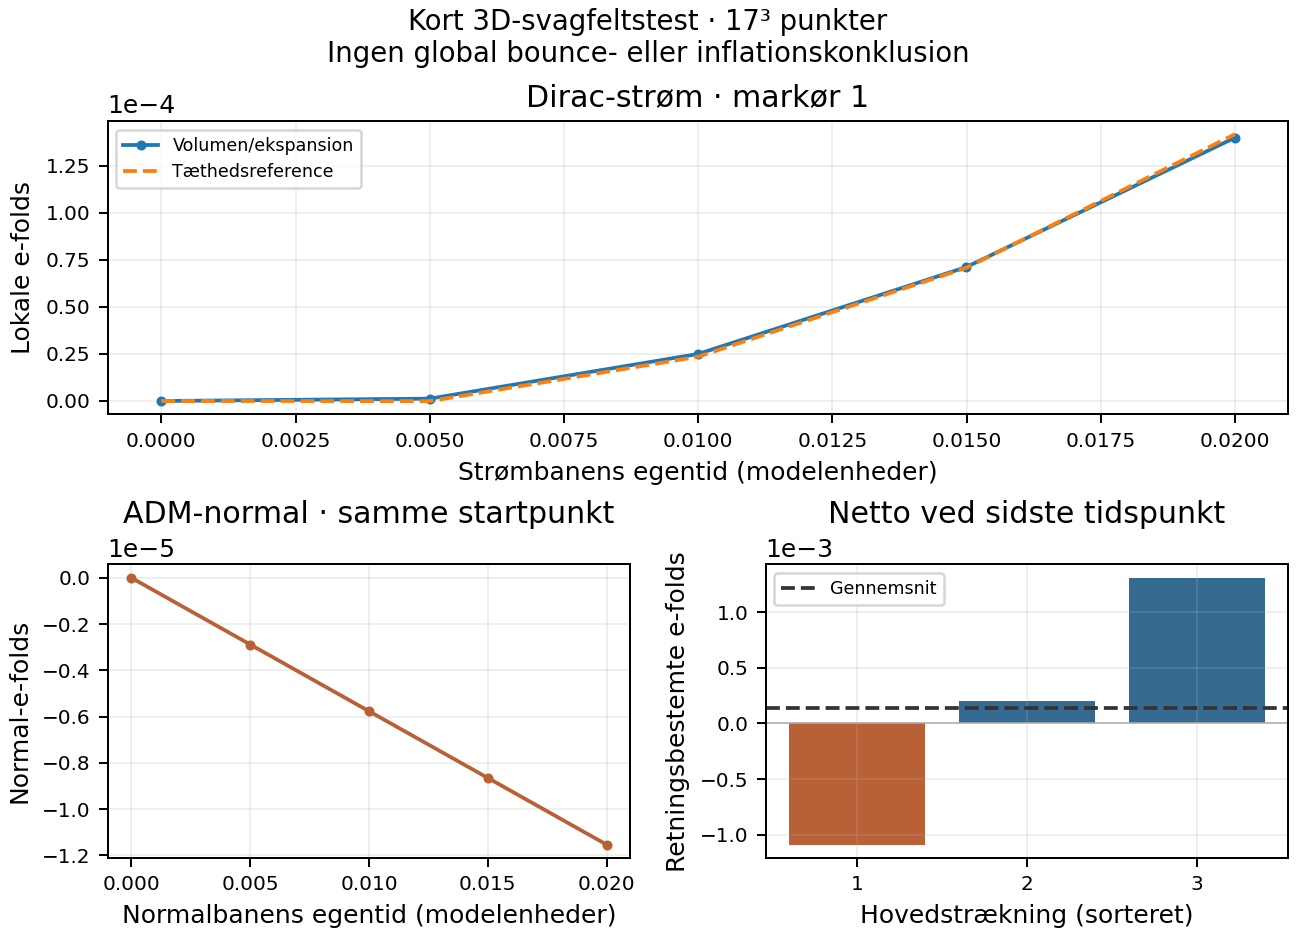
\includegraphics[width=\linewidth]{efolds-example.png}\end{center}}{}

\section{Hvad mangler før det oprindelige kollapsspørgsmål er afgjort?}
Der kræves fysisk begrundede fermiontilstande, globale constrainedata, en konsistent vakuumyderside/randbehandling, stærkfelts- og langtidskonvergens samt kontrolleret fysisk gyldighed. Lokale volumenbounces er ikke det samme som en hel sky, der vender, og heller ikke bevis på, at en dannet sort hul-rumtid undgår singularitet.

For en afgrænset sky skal domæne, massedefinition, start- og slutbegivenheder og observatører fastlægges. Null-udvidelser skal beregnes på faktiske flader; en begivenhedshorisont kræver global kausal information. Der findes ikke en generel sfærisk skalmassesubstitut for ADM-masse.

Undersøgelsen giver dermed generelle eksakte relationer og en kontrollerbar målemetode, men intet universelt antal post-bounce-e-folds. En valideret vending, et no-bounce-resultat for en erklæret klasse eller et uafklaret stop ved gyldighedsgrænsen er alle legitime resultater.

\begin{thebibliography}{9}
\bibitem{HD} Hehl--Datta (1971), doi:10.1063/1.1665738; minimal ikke-lineær Dirac-teori.
\bibitem{G} Gourgoulhon, \href{https://arxiv.org/abs/gr-qc/0703035}{gr-qc/0703035}; ADM.
\bibitem{L} Langlois--Vernizzi, \href{https://arxiv.org/abs/astro-ph/0509078}{astro-ph/0509078v3}, Phys. Rev. D 72, 103501 (2005); geometrisk integreret ekspansion. Perfekt-væske-lukninger overføres ikke til ECD.
\bibitem{B} Buchert--Mourier--Roy, \href{https://arxiv.org/abs/1912.04213}{arXiv:1912.04213v2}, Gen. Rel. Grav. 52, 27 (2020); vilkårlig slicing, tilt og domænevolumen.
\bibitem{M} M\"uller--Nowaczyk, \href{https://arxiv.org/abs/1504.01034}{arXiv:1504.01034v3}; lokal torsionsfri Cauchy-ramme, ikke en global ECD-stabilitetssætning.
\end{thebibliography}
\end{document}
